\chapter{観測、暗黒物質、そして宇宙論的フィット}

\lectureoverview{観測は、宇宙論的モデルと結びつけられて初めて意味を持つ。まずフリードマン方程式と3つの一様な空間幾何学から始め、現在の宇宙の収支を放射、物質、真空エネルギー、曲率に整理し、かつて開いた宇宙が避けられないように思われた理由を再構成する。次に銀河回転曲線が欠落した重力源物質を明らかにし、冷たい弱相互作用ハローの力学へと導く。最後に赤方偏移、明るさ、光源数が、試行的な膨張史を観測可能な曲線へと変える。古い物質＋曲率モデルは失敗し、物質割合が\(0.3\)付近、真空割合が\(0.7\)付近、そして非常に小さな曲率が、この講義の成功したフィットを与える。}

\section{観測を方程式に戻す}

天文的事実は単独では解釈できない。まず、観測のどの組み合わせが一つの宇宙を別の宇宙から区別するのかを教えてくれる方程式が必要である。一様等方な宇宙の出発点はフリードマン方程式であり、
\begin{equation}
\left(\frac{\dot a}{a}\right)^2
=
\frac{8\pi G}{3}\rho-\frac{k}{a^2}.
\label{eq:c06-friedmann}
\end{equation}
量
\begin{equation}
H(t)=\frac{\dot a(t)}{a(t)}
\label{eq:c06-hubble}
\end{equation}
はハッブル\emph{関数}である。その現在値\(H_0\)は慣習的にハッブル定数と呼ばれるが、\(H(t)\)は宇宙史を通じて一定ではない。天文学者がキロメートル毎秒毎メガパーセクで値を示すとき、彼らは\(H_0\)を示しているのである。

規格化された曲率ラベルは3つの値のみを取る。
\begin{equation}
k\in\{+1,0,-1\},
\end{equation}
これはそれぞれ球面、平坦、双曲空間幾何学に対応する。共通のFRW計量は次のように書ける。
\begin{equation}
ds^2=-dt^2+a(t)^2\left[dr^2+\xi(r)^2d\Omega_2^2\right],
\label{eq:c06-frw}
\end{equation}
ここで
\begin{equation}
\xi(r)=
\begin{cases}
\sin r, & k=+1,\\
r, & k=0,\\
\sinh r, & k=-1.
\end{cases}
\label{eq:c06-xi}
\end{equation}
この記法は2つの役割を果たす。3つの幾何学を1つの計量にまとめ、後に球の面積、したがって動径シェル内の光源数を与える。したがって、\(k\)の選択と\(a(t)\)の方程式は、すでに観測的帰結を持つモデルである。

\section{現在の宇宙の収支}

エネルギー密度は、議論中のモデルにおいて3つの主要成分を持つ。放射、非相対論的物質、真空エネルギーである。曲率を同じ収支の行に含めると、
\begin{equation}
\frac{C_r}{a^4}
+\frac{C_m}{a^3}
+\Lambda
-\frac{k}{a^2}
=H^2.
\label{eq:c06-budget}
\end{equation}
ここで\(\Lambda\)は前の講義の規格化\(\Lambda=(8\pi G/3)\rho_{\rm vac}\)を用いている。放射は\(a^{-4}\)として薄まり、物質は\(a^{-3}\)として薄まり、真空エネルギーは薄まらず、曲率は\(a^{-2}\)としてスケールする。曲率は物質的なエネルギー密度ではないが、他の項の隣に置くことで現在の制約が透明になる。すなわち4つの寄与は\(H_0^2\)に足し合わされなければならない。

それらの現在の割合を次で定義する。
\begin{equation}
\begin{aligned}
\Omega_r&=\frac{C_r/a_0^4}{H_0^2},
&\qquad
\Omega_m&=\frac{C_m/a_0^3}{H_0^2},\\
\Omega_\Lambda&=\frac{\Lambda}{H_0^2},
&
\Omega_k&=\frac{-k/a_0^2}{H_0^2}.
\end{aligned}
\label{eq:c06-omegas}
\end{equation}
すると
\begin{equation}
\boxed{\Omega_r+\Omega_m+\Omega_\Lambda+\Omega_k=1.}
\label{eq:c06-sum-rule}
\end{equation}
\(\Omega\)は今日評価された比であり、時間に依存しない定数ではない。また符号の規約に注意せよ。\(k=-1\)は正の\(\Omega_k\)を与える。

\subsection{最初の項はどのように測定されるか}

ハッブルは後退赤方偏移と距離を比較することで局所膨張率を得た。赤方偏移は低\(z\)において速度を与え、較正された明るさは距離を与える。彼の最初の数値はひどく間違っていたが、方法は正しかった。銀河は比較的近くにあったため、測定は宇宙史の大きな割合を探らず、\(H\)をその現在値として扱うことができた。

\begin{classroomqa}
\audiencequestion{内在的な明るさがすでに分かっていなければ、明るさはどうやって距離を決められるのですか。}
\lecturerresponse{一段階ではできない。宇宙距離はしごは近傍星の視差から始まる。その較正された領域にあるセファイド変光星は周期-光度関係を明らかにし、より大きな距離に対する標準光源となる。重なり合う較正がはしごを外側へ運び、超新星は後に用いられる宇宙論的赤方偏移において最良の光源を与える。したがって距離は、すべての天体が等しく輝くという恣意的な仮定からではなく、標準の連鎖から推論される。\lecturetimestamp{00:10:00--00:11:32}}
\end{classroomqa}

\begin{classroomqa}
\audiencequestion{\(C_r\)と\(C_m\)は、それらの密度が変化するのに定数なのですか。}
\lecturerresponse{はい。係数は固定されたままで、因子\(a^{-4}\)と\(a^{-3}\)が時間依存性を担う。真空エネルギーは一定であり、曲率は\(a^{-2}\)としてスケールする。これらの等しくない冪が、まさに割合の寄与が時代ごとに変化する理由である。\lecturetimestamp{00:11:35--00:12:02}}
\end{classroomqa}

放射項は光子背景から局所的に測定できる。その大部分は宇宙マイクロ波背景であり、その現在のエネルギー密度は他の重要な成分に比べてごくわずかである。十分に大きな平均体積が必要だが、\(\Omega_r\)が今日無視できることを確立するために過去の光円錐を長く遡る必要はない。

可視物質は銀河、恒星集団、水素、星間ガスから推定される。方法は概念的には難解というよりむしろ技術的である。すなわち、典型的な恒星とガスの含有量を求め、それを銀河にわたって合計し、大きな体積で平均する。講義では、一立方メートルあたり陽子一個分の質量という古い粗い尺度を引用している。これは放射密度よりはるかに大きいが、それでもなお著しく希薄である。

\begin{classroomqa}
\audiencequestion{この会計では暗黒物質はどうなるのか。}
\lecturerresponse{それはこれから扱うが、まずは発光物質のみに基づく古い推論を意図的に再構成する。歴史的な順序が重要である。それは、暗黒物質がどの見かけの結論を修正したのか、そしてどの隙間を埋めなかったのかを正確に示す。\lecturetimestamp{00:15:08--00:15:40}}
\end{classroomqa}

\section{なぜかつて開いた宇宙が必要と見なされたか}

古い描像では、放射は無視できると正しく判断され、真空エネルギーはゼロに置かれ、物質とは電磁放射を通じて見える物質のみを意味した。得られた推定はおよそ
\begin{equation}
\Omega_r\simeq0,
\qquad
\Omega_\Lambda=0,
\qquad
\Omega_m^{\rm luminous}\sim\frac{1}{20}\text{--}\frac{1}{30}.
\end{equation}
であった。すると和則は
\begin{equation}
\Omega_k\simeq1.
\end{equation}
を強いるように見えた。正の曲率寄与は\(-k/a_0^2>0\)を意味するので、これは\(k=-1\)、すなわち開いた負の曲率の宇宙を意味した。これらの数値は古い議論の再構成であり、現代のパラメータ推定ではない。

曲率スケールを解釈するには、物質支配の解
\begin{equation}
a(t)\propto t^{2/3}.
\end{equation}
に戻る。微分して\(a\)で割ると
\begin{equation}
H(t)=\frac{\dot a}{a}=\frac{2}{3t}.
\label{eq:c06-matter-h}
\end{equation}
が得られる。現在の年齢\(T\)では、
\begin{equation}
H_0\simeq\frac{2}{3T}.
\end{equation}
である。したがってハッブル時間は宇宙の年齢と同じ程度の桁である。放射支配の場合の比較
\begin{equation}
a(t)\propto t^{1/2},
\qquad
H(t)=\frac{1}{2t},
\end{equation}
は、この年齢の逆数関係がダストに特有のものではないことを示している。

\begin{figure}[htbp]
\centering
\includegraphics[width=0.72\textwidth]{lecture_06_figure_02.png}
\caption{物質時代の板書の復習。見える書き込みには\(a\sim t^{2/3}\)と\(\dot a/a=2/(3t)\)が含まれている。講師は残りの板書を隠しているので、隠れた方程式をこのフレームに帰属させることはしない。}
\label{fig:c06-age-board}
\lectureframe{00:24:41.615}
\end{figure}

\begin{classroomqa}
\audiencequestion{ハッブル定数の単位は何か、また光速はどこにあるのか。}
\lecturerresponse{\(H\)は速度を距離に関係づけるので、単位は時間の逆数である。秒の逆数、年の逆数、または天文学者に馴染みのキロメートル毎秒毎メガパーセクで表してよい。関係\(H\sim1/T\)には余分な\(c\)は不要である。\(c\)の因子は、時間\(T\)を\(cT\)のような長さに変換するときにのみ現れる。\lecturetimestamp{00:22:50--00:24:25}}
\end{classroomqa}

ハッブルの当初の値\(H_0\)はおよそ一桁大きすぎたので、対応するハッブル年齢は短すぎ、講義の丸めた比較では百億年ではなく十億年程度であった。より良い較正は数値を修正したが、\(H_0^{-1}\)が宇宙論的な時間尺度であるという論理は変えなかった。

古い曲率の推論は今では
\begin{equation}
\frac{1}{a_0^2}\sim H_0^2\sim\frac{1}{T^2}.
\end{equation}
と読める。単位\(c=1\)では、曲率半径\(a_0\)はしたがって年齢\(T\)の程度と考えられ、通常の単位に戻すと\(cT\)の程度であった。講義は直ちにこれを現実の宇宙についての主張として撤回する。これは、当時無視できると信じられていた項を捨てた後、数十年前に得られた結論である。

\begin{classroomqa}
\audiencequestion{曲率が今日支配すると考えられていたのなら、なぜ物質支配の法則\(a\propto t^{2/3}\)を使うのか。}
\lecturerresponse{物質は\(a^{-3}\)としてスケールするが、曲率は\(a^{-2}\)としてしかスケールしないからである。より小さい\(a\)では物質が勝つ。曲率が重要になり得るのは遅い時期だけなので、物質支配は経過した歴史の大部分を依然として記述し、\(H_0\)を\(1/T\)の程度に保った。完全な混合解は数値因子を修正するだろうが、時間尺度の議論を消し去ることはない。\lecturetimestamp{00:49:20--00:50:17}}
\end{classroomqa}

\section{銀河力学から見た暗黒物質}

物質を目録化する運用上の方法は二つある。一つは光を放出または吸収する物質を数えることである。もう一つは重力から質量を推論することである。オールトは1930年代初頭に銀河の異常な力学を見出し、ツウィッキーは銀河団に類似の質量不一致を見出した。証拠は、重力を及ぼす物質が発光物質を上回ることを示していた。通常の荷電物質は放射し衝突する。欠けている成分は、まずその重力的作用によって知られた。

\begin{classroomqa}
\audiencequestion{発光物質には拡散ガスや中心ブラックホールも含まれるのか。}
\lecturerresponse{拡散ガスは、その量を電磁的振る舞いから推論できる限り含まれる。中心の超大質量ブラックホールは既知の質量収支に含めてよいが、銀河の全質量のほんの一部にすぎず、中心に集中している。発光中心のはるか外側まで続く不一致を説明することはできない。\lecturetimestamp{00:29:50--00:31:14}}
\end{classroomqa}

半径\(r\)のほぼ円軌道を運動する恒星を考える。もし質量\(M\)のほとんどすべてが銀河中心付近に集中しているなら、ニュートンの法則により
\begin{equation}
\frac{GM}{r^2}=\frac{v^2}{r},
\end{equation}
が得られ、したがって
\begin{equation}
v^2=\frac{GM}{r},
\qquad
v(r)\propto r^{-1/2}.
\label{eq:c06-kepler}
\end{equation}
となる。これは中心質量分布の外側で期待されるケプラー的減衰である。

\begin{figure}[htbp]
\centering
\includegraphics[width=0.78\textwidth]{lecture_06_figure_03.png}
\caption{中心質量から囲まれた質量\(M(r)\)への移行における回転曲線の板。\(MG\)、分数の横線、軌道の略図、および曲線の略図の一部のみが見えている。式~\eqref{eq:c06-kepler}は口頭の導出から得られたものである。}
\label{fig:c06-rotation-board}
\lectureframe{00:34:53.642}
\end{figure}

\begin{figure}[htbp]
\centering
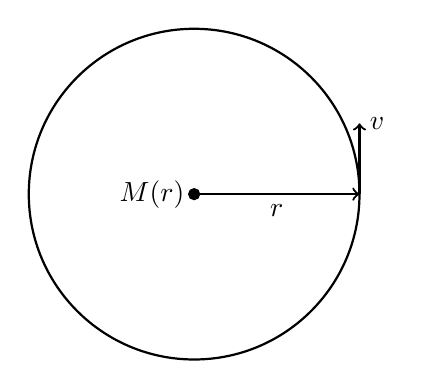
\begin{tikzpicture}[scale=1.0]
\filldraw (0,0) circle (2pt) node[left] {\(M(r)\)};
\draw[thick] (0,0) circle (2.1);
\draw[->,thick] (0,0)--(2.1,0) node[midway,below] {\(r\)};
\draw[->,thick] (2.1,0)--(2.1,0.9) node[right] {\(v\)};
\end{tikzpicture}
\caption{測定された回転速度から囲まれた質量を推測するために用いられた円軌道の構成。}
\label{fig:c06-orbit-redraw}
\end{figure}

観測される銀河回転曲線はこのようには減少しない。かなりの動径範囲にわたって、それらはほぼ平坦である。固定された中心質量を囲まれた質量\(M(r)\)で置き換えると、
\begin{equation}
\frac{G M(r)}{r^2}=\frac{v(r)^2}{r}.
\end{equation}
もし\(v(r)\)がほぼ一定ならば、
\begin{equation}
\boxed{M(r)\propto r.}
\label{eq:c06-enclosed-mass}
\end{equation}
となる。これは半径\(r\)の内側の全質量を指し、局所的な密度を指すのではない。重力を及ぼす質量は、ほとんどの星の光が集中している領域のはるか外側まで増え続ける。銀河円盤に垂直な運動はさらに、ほぼ球対称な分布、すなわち第二の薄い円盤ではなく暗黒ハローを示唆する。

\begin{classroomqa}
\audiencequestion{回転曲線がなぜこれほど平坦なのかを説明する簡単な理論はあるか。}
\lecturerresponse{この議論の中にはない。銀河形成のシミュレーションはそのようなプロファイルを自然なものにするかもしれないが、講義は短い導出を主張してはいない。確実なのは観測的な言明である。すなわち、ほぼ一定の\(v\)は囲まれた質量のほぼ線形な増加を意味する。その関係の整い方を見て、銀河形成の初等的な説明と誤解してはならない。\lecturetimestamp{00:35:58--00:37:33}}
\end{classroomqa}

\begin{classroomqa}
\audiencequestion{渦状腕は、変化する角速度\(v/r\)によって生じる単なる物質の風車なのか。}
\lecturerresponse{単純な風車像は成り立たない。可視のパターンは個々の恒星とともに回転する必要はなく、密度波や星形成波による記述も可能性の一つである。講義はこの不確かさを用いて、頑健なハローの推論と、より複雑な渦状構造の問題とを区別する。\lecturetimestamp{00:37:35--00:38:34; 00:47:03--00:47:47}}
\end{classroomqa}

推測される暗黒質量は光度質量の数倍であり、講義ではおよそ五倍から十倍の間の桁程度の因子としてのみ言及されている。ハローは可視銀河の外側にも広がっている。これらは意図的に粗い歴史的な尺度であり、あらゆる系に当てはまる精密な普遍的な比ではない。

\section{暗黒物質はどのようなものでなければならないか}

なぜ通常の物質は明るくコンパクトな円盤を形成する一方で、暗黒物質は広いハローにとどまるのか。光度をもつ物質は電磁的な衝突と放射を通じて力学的エネルギーを失うことができる。ひとたびエネルギーを散逸すれば、重力はそれをより高密度の配置へ引き寄せることができる。暗黒物質は電気的に中性で、はるかに弱くしか相互作用しないように見える。その粒子はほとんど衝突や放射なしにハローを通り抜けて軌道運動するため、何十億年経っても明るい円盤へ落ち着くのに十分なエネルギーを失わない。銀河の運動による重力放射は、代替の冷却機構を与えるにはあまりにも弱すぎる。

\begin{classroomqa}
\audiencequestion{弱く相互作用するとは、暗黒物質が異なる重力法則に従うという意味か。}
\lecturerresponse{いいえ。それは通常の仕方で重力を及ぼすと仮定されている。ここで弱い相互作用とは、非重力的一衝突と電磁放射が存在しないか、大きく抑制されていることを意味する。二つの暗黒粒子は依然として重力的に引き合う。その引力はハローを組織するが、軌道エネルギーを効率的に散逸させることはない。\lecturetimestamp{00:42:36--00:43:35}}
\end{classroomqa}

\begin{classroomqa}
\audiencequestion{これが一つの銀河回転曲線の特異性にすぎないのではないことを示す観測は何か。}
\lecturerresponse{証拠はいくつかの尺度に現れる。銀河内の恒星運動、銀河面に垂直な運動、銀河間の相互作用、そして銀河団全体の力学である。オールトとツウィッキーの例は、同じ失われた重力の問題の異なる現れであった。\lecturetimestamp{00:42:00--00:42:36}}
\end{classroomqa}

\begin{classroomqa}
\audiencequestion{暗黒物質はブラックホールや銀河中心の周りに集まるべきか。}
\lecturerresponse{それは重力中心に向かってより高密度になるが、歴史的な順序は、既存のブラックホールの周りにハローが形成されるという逆のものである可能性が高い。暗黒ハローが大きな重力の井戸を形成し、その後バリオン物質がそれらに落ち込んで銀河、恒星、中心ブラックホールを形成した。ブラックホールは質量の小さな部分である。それでも対消滅生成物の探索が銀河中心に向けられるのは、そこでは暗黒物質の密度がより高いと予想されるからである。\lecturetimestamp{00:43:36--00:45:43}}
\end{classroomqa}

\begin{classroomqa}
\audiencequestion{暗黒物質は気体、塵、コンパクトな塊、それとも孤立した粒子なのか。その一部は太陽の近くに捕らえられている可能性があるか。}
\lecturerresponse{その微視的性質は不明であるが、通常の塵は電磁気力によって束縛されており、これはまさに暗黒物質が欠いているように見える種類の相互作用である。したがって既定の粒子像は、個々の粒子が希薄に分布した集団である。一部は重力によって太陽の近くに集中しているかもしれないが、その密度は太陽重力と競合したり惑星の力学を乱したりするにはあまりにも小さすぎる。\lecturetimestamp{00:45:43--00:47:02; 00:58:41--00:59:29}}
\end{classroomqa}

第二の中心的要件は、暗黒物質が集積することである。相対論的な無作為速度をもつ高温の集団は重力による集積に抵抗し、低温の集団はポテンシャル井戸に落ち込むことができる。通常の軽いニュートリノは高温暗黒物質として振る舞ったはずであり、必要とされる銀河の主要成分を与えない。この文脈で\emph{低温}とは、局所的な宇宙論的座標系において非相対論的であることを意味し、文字どおり実験室の絶対零度にあることを意味するのではない。

\begin{classroomqa}
\audiencequestion{低温で集積するという要件は、暗黒物質の質量範囲を課すのか。}
\lecturerresponse{それは量子統計と生成の履歴に依存する。非常に軽いフェルミオンはすべてが一つの遅い状態を占めることはできず、強く制約される。非常に軽いボソンはコヒーレントなボース凝縮状態を占めることができ、アクシオンが講義における例である。あるいは、より重い弱い相互作用をする粒子は凝縮なしに低温でありうる。したがって、この議論から与えられるモデルに依存しない単一の質量限界は存在しない。\lecturetimestamp{00:53:17--00:54:52; 00:56:42--00:58:05}}
\end{classroomqa}

\begin{classroomqa}
\audiencequestion{加速器はすでにこれらの粒子を発見しているべきではないのか。}
\lecturerresponse{それは追加の仮定の下でのみである。粒子がおおよそ弱い相互作用の断面積をもち、質量が加速器の到達範囲内にあれば、衝突型加速器での生成が可能かもしれない。差し迫った情報が得られるという講義の期待は明示的に推測的であり、歴史的に時代遅れのものであった。代わりに、粒子が重すぎたり、利用可能な実験に対して弱くしか相互作用しなかったりする可能性もある。\lecturetimestamp{00:54:52--00:55:54}}
\end{classroomqa}

\begin{classroomqa}
\audiencequestion{暗黒物質は見えない余剰次元に住んでいるだけではないのか。}
\lecturerresponse{この議論ではそのような機構は必要ない。暗黒物質はすでに重力的に観測されており、通常の物質とほとんど相互作用しない風変わりな粒子から単に成り立っているのかもしれない。相互作用を弱いと呼ぶことは、粒子を観測可能な時空の外に置くことと同じではない。\lecturetimestamp{00:55:54--00:56:41}}
\end{classroomqa}

見えない物質を加えるのではなく重力を修正することは、論理的な代替案である。講義は、当時、関連するすべてのスケールにわたる証拠を説明しつつ、成功した太陽系の法則を保持する、同程度に単純な修正は存在しなかったと判断している。したがって粒子解釈が好まれるが、その微視的物理学は依然として不明である。

\section{暗黒物質は古い収支を閉じない}

暗黒物質は物質の寄与を数倍に拡大するが、発光物質と\(H_0^2\)の間の古い不一致はおよそ二十五の桁であった。したがってそれは隙間を狭めるが、
\begin{equation}
\frac{C_m}{a_0^3}=H_0^2.
\end{equation}
にはしない。古い\(\Lambda\)なしの描像の内部では、正の曲率収支項、したがって\(k<0\)が依然として必要であった。そのような開いたモデルに論理的な矛盾は何もなかった。要点は、暗黒物質だけでは現代の答えを選び出さなかったということである。

\begin{classroomqa}
\audiencequestion{現代のフィット以前に、宇宙論者たちは曲率について実際に何を考えていたのか。}
\lecturerresponse{証拠は混乱しており、閉じた有界な宇宙への事前の選好が物質収支に反して引っ張ることがあった。古い仮定を一貫して組み合わせると、負の曲率が自然な推論であった。その歴史的な合意は依然として暫定的なものであった。なぜなら、暗黒物質も真空エネルギーも、今日のような仕方で確実に組み込まれていなかったからである。\lecturetimestamp{00:50:17--00:51:50}}
\end{classroomqa}

したがって我々は、一つの収支の行からその真偽を推論するのではなく、候補モデルを検証しなければならない。モデルは曲率の選択\(k\)と膨張史\(a(t)\)、等価的には物質の状態方程式の組と、そこから\(a(t)\)が計算される現在のパラメータから成る。古い候補は、放射を無視でき宇宙定数をもたない、物質と負の曲率である。

\section{幾何学を観測量に変える}

\subsection{凍結された幾何学における光源数と明るさ}

一時的に宇宙の進化を無視する。一様な宇宙では、共動殻内の光源の数はその面積に比例する。
\begin{equation}
dN\propto \xi(r)^2\,dr.
\label{eq:c06-shell-count}
\end{equation}
したがって
\begin{equation}
dN\propto
\begin{cases}
\sin^2r\,dr, & k=+1,\\
r^2\,dr, & k=0,\\
\sinh^2r\,dr, & k=-1.
\end{cases}
\end{equation}
大きな\(r\)では、負の曲率の場合\(\sinh^2r\sim e^{2r}\)として増大し、平坦な\(r^2\)則よりもはるかに速い。したがって負の曲率は、距離とともに光源の数が異常に急速に増加することを予測する。

同じ面積が受けるフラックスを決める。平坦で静的な空間では、標準的な光源は
\begin{equation}
F\propto\frac{1}{r^2}.
\end{equation}
を与える。双曲空間では放射が広がる球面がより速く成長するため、フラックスはより速く減少する。講義ではこの観測量を光度と呼ぶことがあるが、ここで\(F\)は明るさすなわちフラックスを表し、固有の光度は光源に属する。したがって、計数と明るさを合わせれば空間幾何を区別できる。

\subsection{赤方偏移と過去光円錐}

現実の宇宙は進化しており、外を見ることは時間を遡って見ることを意味する。\(t_{\rm em}\)で放出された光は、スケール因子が\(a(t_{\rm em})\)から\(a_0\)へ成長する間に引き伸ばされる：
\begin{equation}
1+z
=\frac{\lambda_{\rm obs}}{\lambda_{\rm em}}
=\frac{a_0}{a(t_{\rm em})}.
\label{eq:c06-redshift}
\end{equation}
同値な形では、
\begin{equation}
z=\frac{\lambda_{\rm obs}}{\lambda_{\rm em}}-1.
\end{equation}
我々の過去光円錐に沿った異なる点は、同時に異なる共動半径と異なる放出時刻に対応する。膨張は波長を変える。ドップラー偏移と重力偏移は別の物理的機構であるが、ここで問題となっている効果は宇宙論的膨張である。

\begin{classroomqa}
\audiencequestion{なぜ\(z\)の定義にはマイナス1が含まれるのか。}
\lecturerresponse{これは、偏移を受けていない光源が\(z=0\)となるように選ばれた歴史的な慣習である。物理的に直接的な伸長因子は\(1+z=\lambda_{\rm obs}/\lambda_{\rm em}\)である。\lecturetimestamp{01:10:11--01:10:45}}
\end{classroomqa}

動径方向の光は\(d\Omega_2=0\)であり、\(ds^2=0\)に従う。したがって式~\eqref{eq:c06-frw}は
\begin{equation}
dt^2=a(t)^2dr^2.
\end{equation}
を与える。我々から逆向きにたどる入射光線に対しては、
\begin{equation}
dt=-a(t)\,dr,
\qquad
\frac{dr}{dt}=-\frac{1}{a(t)}.
\label{eq:c06-null-ray}
\end{equation}
マイナス符号は、光線に沿ってより大きな共動半径がより早い時刻にあることを示す。\(a(t)\)が分かれば、この式が\(r(t)\)を決定する。

\subsection{赤方偏移当たりの数}

観測者は標準光源を赤方偏移ビン\(z\)から\(z+dz\)まで数えることができる。式~\eqref{eq:c06-shell-count}から始め、過去光線に沿って式~\eqref{eq:c06-redshift}を微分すると、
\begin{equation}
dz=-\frac{a_0}{a^2}\,da
=-\frac{a_0}{a^2}\dot a\,dt.
\end{equation}
\(dt=-a\,dr\)を用いると、
\begin{equation}
dz=\frac{a_0}{a}\dot a\,dr
=(1+z)\dot a\,dr.
\end{equation}
したがって
\begin{equation}
dr=\frac{dz}{(1+z)\dot a},
\end{equation}
であり、共動光源密度が固定されている場合、
\begin{equation}
\boxed{
\frac{dN}{dz}
\propto
\frac{\xi(r)^2}{(1+z)\dot a}
}.
\label{eq:c06-dndz}
\end{equation}
となる。実演による導出では符号と因子が何度も確認される。式~\eqref{eq:c06-null-ray}\allowbreak と\allowbreak\eqref{eq:c06-redshift}\allowbreak が結果を一義的に定める。

\begin{figure}[htbp]
\centering
\includegraphics[width=0.84\textwidth]{lecture_06_figure_05.png}
\caption{黒板上の\(dN/dz\)とモデル関数との関係。左辺と右辺の\(a\sim t^{2/3}\)、\(\dot a\)、\(r(t)\)は見えるが、講師が分母の一部を隠している。式~\eqref{eq:c06-dndz}は上で独立に確立されている。}
\label{fig:c06-dndz-board}
\lectureframe{01:22:24.114}
\end{figure}

モデルを選ぶまではこれ以上評価すべきものはない。指定された\(a(t)\)が\(\dot a(t)\)を決定し、式~\eqref{eq:c06-null-ray}が\(r(t)\)を決定し、式~\eqref{eq:c06-redshift}によってすべての量を\(z\)で表せる。異なる状態方程式は異なる関数\(dN/dz\)と\(F(z)\)を生む。まさにこのことが観測を識別的にする。

\section{試行パラメータから最良適合へ}

手順は直接的である：
\begin{equation}
(\Omega_r,\Omega_m,\Omega_\Lambda,\Omega_k)
\longrightarrow
a(t)
\longrightarrow
\left\{F(z),\frac{dN}{dz}\right\}.
\label{eq:c06-fit-pipeline}
\end{equation}
現在のパラメータを選び、フリードマン方程式を解き、動径方向の光を伝播させ、赤方偏移に対する明るさと計数を計算し、曲線をデータと比較する。比較に失敗すればそのパラメータ集合は棄却される。二つの観測量を合わせることで、膨張史と空間幾何の両方が制約される。

\begin{figure}[htbp]
\centering
\includegraphics[width=0.84\textwidth]{lecture_06_figure_06.png}
\caption{上側の黒板には古い物質＋曲率モデル、下側の黒板には平坦および双曲のシェル因子\(r^2dr\)と\(e^{2r}dr\)がある。フリードマン方程式の一部が覆われているため、このフレームは方程式の出典ではなく補助的証拠である。}
\label{fig:c06-old-model-board}
\lectureframe{01:24:27.863}
\end{figure}

古いモデル、
\begin{equation}
H^2=\frac{C_m}{a^3}-\frac{k}{a^2},
\qquad k=-1,
\end{equation}
は明るさ–赤方偏移関係と光源計数の両方のテストに失敗する。超新星は、関係する赤方偏移範囲で最も有用な標準光源を提供する。講義の成功したパラメータ集合は
\begin{equation}
\boxed{
\Omega_r\simeq0,\qquad
\Omega_m\simeq0.3,\qquad
\Omega_\Lambda\simeq0.7,\qquad
\Omega_k\simeq0
}.
\label{eq:c06-best-fit}
\end{equation}
である。ここでの物質には輝く物質と暗黒物質が含まれる。これらの値は講義当時の適合を報告するものであり、持続する教訓は適合の方法と、希薄化しない支配的成分の必要性であって、最後に印刷された小数ではない。

\subsection{何が測定され、何が適合されるかについての質問}

\begin{classroomqa}
\audiencequestion{古い開いた宇宙モデルを議論している間に\(\Lambda\)はすでに仮定されていたのか。}
\lecturerresponse{いいえ。最初の部分では\(\Lambda=0\)として古いモデルを意図的に再構成した。式~\eqref{eq:c06-best-fit}の値は後の現代的な適合を記述する。古い候補は黙って修正されたのではなく、\(F(z)\)と\(dN/dz\)に対して検証され、失敗した。\lecturetimestamp{01:26:45--01:27:07}}
\end{classroomqa}

\begin{classroomqa}
\audiencequestion{真空エネルギーが局所的な物質のように直接測定されないのなら、\(\Omega_\Lambda\)はどのようにして得られるのか。}
\lecturerresponse{試行的なパラメータ集合から始める。各集合は一つのフリードマン解を定義し、したがって予測関数\(F(z)\)と\(dN/dz\)を定める。それらの予測を観測と比較し、適合の悪いものを捨て、パラメータ空間の最良の領域を保持する。数値\(0.7\)はフィットからの推論であり、真空エネルギー計からの直接の読み取りではない。\lecturetimestamp{01:27:08--01:29:59; 01:31:57--01:33:40}}
\end{classroomqa}

\begin{classroomqa}
\audiencequestion{現在のスケール\(a_0\)はどこから来るのか。}
\lecturerresponse{\(a\)の規格化は部分的に慣習的であるが、\(H_0\)に結びついた完成した模型は、\(k\ne0\)のとき現在の物理的な曲率スケールを与える。模型が赤方偏移の観測量に適合すれば、その関数\(a(t)\)が現在の点と対応するスケールを特定する。\lecturetimestamp{01:29:59--01:30:42}}
\end{classroomqa}

\begin{classroomqa}
\audiencequestion{何十億年も過去を覗くことは、今日のパラメータに基づくフィットを歪めるのか。}
\lecturerresponse{過去への遡及は歪みではなく、それこそが信号である。今日のパラメータはフリードマン方程式に代入され、方程式がそれらを完全な\(a(t)\)へと発展させる。予測される光円錐は、より小さな\(a\)では物質がより重要であったこと、そして十分に過去では放射が支配することをすでに含んでいる。この進化を無視する模型はデータに適合しないであろう。\lecturetimestamp{01:30:43--01:31:55}}
\end{classroomqa}

\begin{classroomqa}
\audiencequestion{どの現在の量が比較的直接に測定されるのか。}
\lecturerresponse{放射密度は測定されており、今日では無視できる。ハッブル率は距離と赤方偏移の関係から測定される。全物質密度は、発光物質と暗黒物質を含めて重力的に推論され、臨界スケール\(3H_0^2/(8\pi G)\)で割って\(\Omega_m\)を得る。残る晩期の自由度は主に真空エネルギーと曲率にある。\lecturetimestamp{01:33:40--01:35:32}}
\end{classroomqa}

\begin{classroomqa}
\audiencequestion{\(\Omega_\Lambda\)と\(\Omega_k\)の両方が未知であるのに、\(\Omega_m\)を固定した後、晩期の独立な試行パラメータが一つしかないのはなぜか。}
\lecturerresponse{方程式~\eqref{eq:c06-sum-rule}が一つの拘束条件を課すからである。\(\Omega_r\)が無視でき、\(\Omega_m\)が測定されているとき、試行\(\Omega_\Lambda\)を選ぶと残りの\(\Omega_k=1-\Omega_m-\Omega_\Lambda\)が定まる。同じ一次元族を曲率でパラメータ化してもよい。例えば、\(\Omega_m=0.3\)のとき\(\Omega_\Lambda=0.4\)かつ\(\Omega_k=0.3\)は有効な試行である。それが棄却されるのは、予測曲線の適合が悪いからにすぎず、和則がそれを禁じるからではない。\lecturetimestamp{01:35:33--01:39:09}}
\end{classroomqa}

\begin{classroomqa}
\audiencequestion{\(\Omega_k\)が連続的に変化するのに、\(k\)が\(+1,0,-1\)のみでありうるのはなぜか、また次元は正しいのか。}
\lecturerresponse{離散的な\(k\)は符号と規格化された幾何のみを記録する。連続的な曲率半径は\(a_0\)が担うので、\(-k/(a_0^2H_0^2)\)は連続的な値を取りうる。単位\(c=1\)では、逆長さと逆時間は同じ次元をもつ。通常の単位に戻すと、必要な\(c\)の冪が供給される。\lecturetimestamp{01:39:10--01:40:07}}
\end{classroomqa}

\begin{classroomqa}
\audiencequestion{銀河種族が進化するのに、計数法は一様性と等方性を仮定するのか。}
\lecturerresponse{十分に大きなスライス上での空間的一様性と等方性を仮定しており、それらの対称性は同じ赤方偏移で異なる方向を比較することによって検証できる。光源の進化は別の問題である。異なる時代の種族は同一である必要はないので、実際の解析では数密度が永遠に固定されているふりをするのではなく、選択と進化を模型化する。単純な導出は、それらの洗練を加える前に幾何因子を分離する。\lecturetimestamp{01:40:08--01:41:08}}
\end{classroomqa}

\section{密度分率は進化する}

方程式~\eqref{eq:c06-budget}はあらゆる時刻で成り立つが、方程式~\eqref{eq:c06-omegas}における\(\Omega\)は現在時刻で定義されたものであった。それらの時間依存の類似物は、四つの項が\(a\)の異なる冪をもつために変化する。はるか過去では、
\begin{equation}
\Omega_r(t)\longrightarrow1.
\end{equation}
放射がより速く薄まるにつれて、物質が支配へと近づいて増大する。その後、物質自体が薄まる一方で\(\Lambda\)は固定されたままなので、はるか未来では、
\begin{equation}
\Omega_\Lambda(t)\longrightarrow1.
\end{equation}
したがって物質分率は小さく始まり、物質時代にはほぼ1に近づき、真空エネルギーが取って代わった後に再び減少する。曲率は、非零であれば、最終的には正の定数\(\Lambda\)にも負ける。

\begin{classroomqa}
\audiencequestion{現在の曲率の割合が小さいということは、宇宙が膨張するにつれて平坦になっていくという意味ですか。}
\lecturerresponse{その物理的な曲率スケールは\(a\)とともに増大し、正の宇宙定数に対して曲率の寄与\(a^{-2}\)はますます重要でなくなる。これが\emph{大きいことは平坦である}という表現の意味である。これは離散的なトポロジーのラベル\(k\)を変えるものではない。局所的な曲率と、曲率の力学的な重要性の割合が減少することを述べているのである。\lecturetimestamp{01:47:13--01:47:42}}
\end{classroomqa}

\begin{classroomqa}
\audiencequestion{フィットされたモデルは説明できない系統的な残差を示したのか、またその主張はどの程度精密だったのか。}
\lecturerresponse{講義は、その水準でこの枠組みに知られた系統的な破綻はないと報告し、それをおよそパーセントスケールの精密宇宙論であり、十分の一パーセントや百分の一パーセントではないと述べている。その記述は歴史的なものであり、時代を超えた現在の誤差幅に置き換えるべきではない。\lecturetimestamp{01:45:40--01:46:19}}
\end{classroomqa}

\begin{classroomqa}
\audiencequestion{空間曲率は、超新星の明るさと計数だけによってではなく、直接的な三角測量によって検証できるのか。}
\lecturerresponse{できる。宇宙マイクロ波背景放射の角度パターンは標準的な物理スケールを与え、したがって大きな宇宙的三角形を与える。超新星のデータだけでは、講義のパーセント水準の曲率に関する完全な主張は得られなかった。それらをマイクロ波背景放射の幾何学と組み合わせることで、検証は鋭くなった。これが次の講義の主題である。\lecturetimestamp{01:46:19--01:47:12}}
\end{classroomqa}

\section{持ち越すべきこと}

中心的な教訓は四つの数の目録ではない。それは方法である。宇宙論的パラメータの組は\(a(t)\)を生み出す。すると計量が光の伝播、光源の明るさ、光源の計数を予測する。一致は、選ばれたパラメータと、それらを結びつけるフリードマンの枠組みの両方を検証する。任意の組が必ずフィットする理由はない。

古い、光度を持つ物質と負の曲率のモデルは失敗した。暗黒物質は重力を及ぼす物質の目録を修復したが、それ自体では古いフリードマンの収支を閉じなかった。講義の時代に成功したフィットにはおよそ
\begin{equation}
\Omega_m\simeq0.3,
\qquad
\Omega_\Lambda\simeq0.7,
\qquad
\Omega_k\simeq0,
\end{equation}
が必要であり、その曲率の精度は重要な点でマイクロ波背景放射に依存していた。このモデルが信頼できるのは、いくつかの独立な観測が一つの力学理論を通り、パラメータ空間の同じ領域で出会うからである。
